\documentclass{article}
\usepackage{graphicx} % Required for inserting images
\graphicspath{{images/}}
\usepackage[utf8]{inputenc}
\usepackage{amsmath}
\usepackage{blindtext}
\usepackage{setspace}
\doublespacing
\usepackage{geometry}
\usepackage{natbib}
\usepackage{graphicx}
\usepackage{subcaption}
\usepackage{soul}
\usepackage{multicol}
\usepackage[capposition=top]{floatrow}
\usepackage{booktabs}
\usepackage{appendix}
\usepackage{rotating}
\usepackage{chngcntr}
\usepackage{blindtext}
\usepackage{hyperref}
\usepackage[english]{babel} % for assumption text
\newtheorem{assumption}{Assumption}
% \usepackage{subfiles}

\DeclareRobustCommand{\firstsecond}[2]{#1}


\title{When the Hot-Hand Turns Cold: Responses to streaks of inaccurate forecasts\footnote{I thank John Chalmers at the University of Oregon for providing access to the \citeauthor{Nielsen} Datasets. This paper represents the researcher's own analyses calculated (or derived) based in part on data from Nielsen Consumer LLC and marketing databases provided through the NielsenIQ Datasets at the Kilts Center for Marketing Data Center at The University of Chicago Booth School of Business. Conclusions drawn from the NielsenIQ data are those of the researcher and do not reflect the views of NielsenIQ. NielsenIQ is not responsible for, had no role in, and was not involved in analyzing and preparing the results reported herein}}
\author{\href{https://www.micaelawood.com/}{Micaela D. Wood}\footnote{Email: mwood13@uoregeon.edu Website: micaelawood.com}}
%\date{\today}

\begin{document}

\maketitle

\begin{abstract}
When making decisions involving response and preparation for hurricanes and other disasters, individuals must determine how much risk they are willing to accept, and how much risk they believe they will face. There are many factors that can drive perceptions of risk. Notable drivers of risk perception are recency bias, and the hot-hand fallacy. Using the results of past hurricane forecasts and sales of emergency supplies, I find that responses to hurricane forecasts are largely influenced by past both recency bias and the hot-hand fallacy. Panic buying is significantly larger in counties with inaccurate most recent forecasts, and panic buying continues to get marginally worse as inaccurate forecasts are repeated.
\end{abstract}

\section{Introduction}

Natural disasters require individuals to take on some level of risk. Disasters that can be forecast, like hurricanes, allow individuals to gather information to determine how much risk they believe they will face and allow individuals time to prepare for this perceived risk. There is an extensive literature on risk and its perception in many facets of the economy from financial markets, \citep{rigotti2005uncertainty,gokhale2015misvaluation, rabbani2020financial} to climate and disasters, \citep{gallagher2014learning, bakkensen2019flood, burke2022exposures} to gambling \citep{ladouceur1995cognitive, studer2015put, durand2021behavioral}. In all branches that focus on risk, there is discussion of various fallacies and biases that people fall victim to. Given these biases show up in so many aspects of decision making, it is natural that they may also occur when facing the risk of natural disaster forecasts. 

Two prominent biases in decision making are the recency bias and the hot-hand bias. Both biases occur when individuals place undue weight on prior results rather than the individual probabilities. Recency bias is occurs whenever individuals place high weight on a specific outcome occurring, simply because it occurred recently, regardless of the actual probability \citep{gallagher2014learning, rabbani2020financial, metz2023high, huseynov2025role}. With hurricanes, individuals may be less inclined to believe that a current hurricane forecast for the area will affect them, if the last forecast resulted in the same. Such behavior would be undesirable on a large scale. People less inclined to believe a forecast not prepare sufficiently, or wait until the last minute to do so. Both outcomes could further increase the already high costs of disaster recovery \citep{NorrisEtAl99,SattlerEtAl00,Baker11,deryugina2017fiscal,beatty2019disaster}.

The hot-hand fallacy occurs whenever people believe that a certain independent outcome will occur with high probability because there is currently a streak of the specific outcome, \citep{croson2005gambler, stockl2015hot, studer2015put, miller2024cold}. In hurricane forecasting, there are few streaks of accurate forecasts, all relatively short. Inaccurate forecasts occur more often and streaks last for longer. Based on current literature, it is expected that individuals will be less likely to believe that a streak of accurate results will continue. Inaccurate streaks could however be so long that individuals start by overreacting but eventually stop reacting to forecasts at all \citep{rabin2010gambler}. Overreacting to a forecast does not impose any inherent danger to individuals, but is not efficient. Underreacting or not reacting at all, on the other hand, could be potentially hazardous.

I utilize historic hurricane forecast data from the National Oceanic and Atmospheric Administration (NOAA) along with NielsenIQ Retail Scanner Data on sales of bottled water to test for both recency bias and the hot-hand fallacy. I find that there is strong evidence of recency bias. If the prior hurricane forecast was inaccurate, sales of bottled water are 16 percentage points higher than if the prior forecast was accurate. This effect holds with various definitions of a current hurricane forecast. 
Using various definitions of a streak, I also find significant evidence of recency bias. As a streak of accurate forecasts increases, there is a significant reduction in sales of bottled water, indicating a reduction in panic buying. However, as streaks of inaccurate forecasts get longer, sales of bottled water begin by increasing, and then around 15 incorrect forecasts in a row, they begin to decrease. Once the streak of incorrect forecasts reaches 30, sales of emergency supplies no longer respond to current hurricane forecasts. 

The effects of recency bias and the hot-hand fallacy would both be reduced under more consistently accurate forecasts. To show the impacts of increased forecasting technology, I estimate the change in sales of bottled water that would occur from an improved forecast history. By comparing the expected sales from a hurricane under the current and improved forecast records, it is clear that the hot-hand behavior would be reduced. Counties which currently have streaks of 15 or more inaccurate forecasts would increase their purchases of bottled water by up to \$4,700 per 100 thousand residents. Counties with current streaks less than 15 inaccuracies would see reduced sales of bottled water of up to \$8,250 per 100 thousand residents. Thus improved forecasting technology would like lead to more consistent preparation and reduced panic buying for the majority of coastal counties. 

Much work has been done in the natural disaster literature on the market effects after a disaster occurrence \citep{groen2008effect,semenza2011climate,deryugina2017fiscal,deryugina2018economic,sytsma2020impact}. Many have also shown that panic buying of natural disasters occurs frequently before natural disasters even though this is an undesirable effect\citep{NorrisEtAl99,Baker11,beatty2019disaster}. There is still little understood about what effects panic buying behavior. Because hurricane landfalls are massively destructive events \cite{DisasterCosts}, but also have a variance in their forecasts,the general population faces large amounts of uncertainty during hurricane forecasts. I utilize past forecast tracks and end results to test for signs of the population using their prior experience to determine how they will prepare for disasters today. I find significant evidence that the majority of the panic buying decision is based on past forecast accuracy rather than the current forecasts

Recency bias in the climate change literature has primarily focused on larger purchases immediately following a disaster \citep{hallstrom2005market,gallagher2014learning, bakkensen2019flood} or on surveys between events \cite{kelly2012evolution, MeyerEtAl14}. By using sales data across many years, I am able to follow patterns before and after many different events. This gives me large power in my calculations and the ability to determine that not only does the population respond differently to past forecasts based on whether or not they were correct. The general population is far more likely to panic buy supplies when the last forecast resulted in no hurricane landfall. The implications of this behavior could further help businesses and government to determine which areas will have stronger demands for emergency supplies in the future.

Literature on the hot-hand fallacy has primarily focused on gambling, sports, and financial markets \cite{croson2005gambler,rigotti2005uncertainty,rabin2010gambler,stockl2015hot,studer2015put}. There has been little work outside on these specific areas. By testing for the hot-hand in  natural disaster prep, I show that the hot-hand fallacy extrapolates to nontraditional risk environments. Additionally, hot-hand studies primarily only focus on streaks in one-direction (i.e. bets on a team with a win streak \citep{durand2021behavioral}). Hurricane forecasts over the last decade have had both streaks of accurate forecasts and inaccurate forecasts. I take advantage of this unique scenario to show the novel result that the hot-hand fallacy holds not only for streaks of positive outcomes, but also for streaks of negative outcomes.

The remainder of the paper proceeds as follows. Section II discusses the data and variable creation. Section III discusses the methodology while section IV reports the results. I conclude with section V. 

\section{Data}

\subsection{Sales Data}

To measure responses to hurricane forecasts, I analyze sales of emergency supplies using \citeauthor{Nielsen} Retail Scanner Data. The data records sales from various stores throughout the country, and has coverage in almost every southeastern county. These sales figures include the average weekly price for each product, how many were sold in a given week, and which county the store is located in. By combining the stores in a county, I calculate the weekly total revenue for each product. 

There are a variety of items recommended by the Department of Homeland Security to keep on hand when living in a Natural Disaster prone location. Some items are quite durable and rarely purchased, such as flashlights or hand radios leading or little variation in sales over time. Others have broad definitions that lead to strong taste preferences, such as non-perishable ready-to-eat foods, leaving room for large variation from one geographical location to another of what people may prefer to keep on hand. This makes it difficult to extrapolate any potential results. I choose to focus on sales of bottled water as a way to measure reactions. Bottled water is a consumable good that is accessible at a variety of stores, cheap enough for nearly any household to purchase, and relies less on tastes and preferences, making it an ideal product for analysis.

%Stats on water sales as a whole and around hurricanes.

\subsection{Hurricane Forecast Data}

NOAA records past hurricane forecasts since 2008 in their GIS Archive (\citeauthor{NOAAGIS}). Each tropical cyclone on record since 2008 is recorded along with every advisory update since a strom's inception. Each advisory includes the storms current location, the center of its projected path for the next five day, the projected cone of uncertainty, as well as current and projected windspeed. Using this data, I can see exactly how the hurricane forecast was preseneted to the general public at differet points in time. 

Since tropical advisories are updated every six hours, there are four advisories in a single day. To see if a county is under threat of a hurricane, I test if any portion of a county overlapped the ``cone of uncertainty'' during each advisory. If a county is overlapped by the cone during at least one advisory on that day, it is considered threatened. This accounts for movement of the hurricane parrallel to the coast. Additionally, counties may fall into different timing of a potential threat. As the hurricane moves closer to shore, the number of days until landfall for counties may also change. Because hurricanes may land at any point, it is quite feasible for a county to start a day with a hurricane expected in four days, and end the day with the hurricane expected in three days. To reflect this, I allow counties to fall under multiple day-out threat levels during a single calander day. 

To align with the sales data, I aggregate the daily forecasts to a weekly level. Becuase a hurricane may land during any day of the week, and forecasts are at most five days prior, it is possible for the landfall and forecasts to all fall during the same week, or for all forecasts to be during the week prior to landfall. To avoid any loss of information, I create variables to indicate if a county was under a specific timing of threat (i.e. three days until expected landfall) from one day to five days. Then I create the aggregate variable to indicate if the county was under a threat of any type by summing the daily threat variables. 

To study the impact of the most recent hurricane forecast, I must determine which forecasts where accurate or not. I build three definitions for final forecast type: hurricane forecast resulting in a landfall, hurricane forecast with no landfall, and landfall without any prior forecast. The third class of forecast is exceptionally rare with only one significant occurence from 2008 to 2019. Due to this, I focus on the first two definitions which will respectively be called hit and miss for simplicity. 

To estimate the effects of any recency bias, I need the results of the most recent prior hurricane forecast. Simply put, once a county has their first hurricane forecast in the data, the result gives their most recent forecast result, hit or miss,  from the next week onward. Once a new hurricane has been forecast and the result defined, the most recent forecast data is replaced with the new result. 

\begin{figure}[!t]
    \centering
    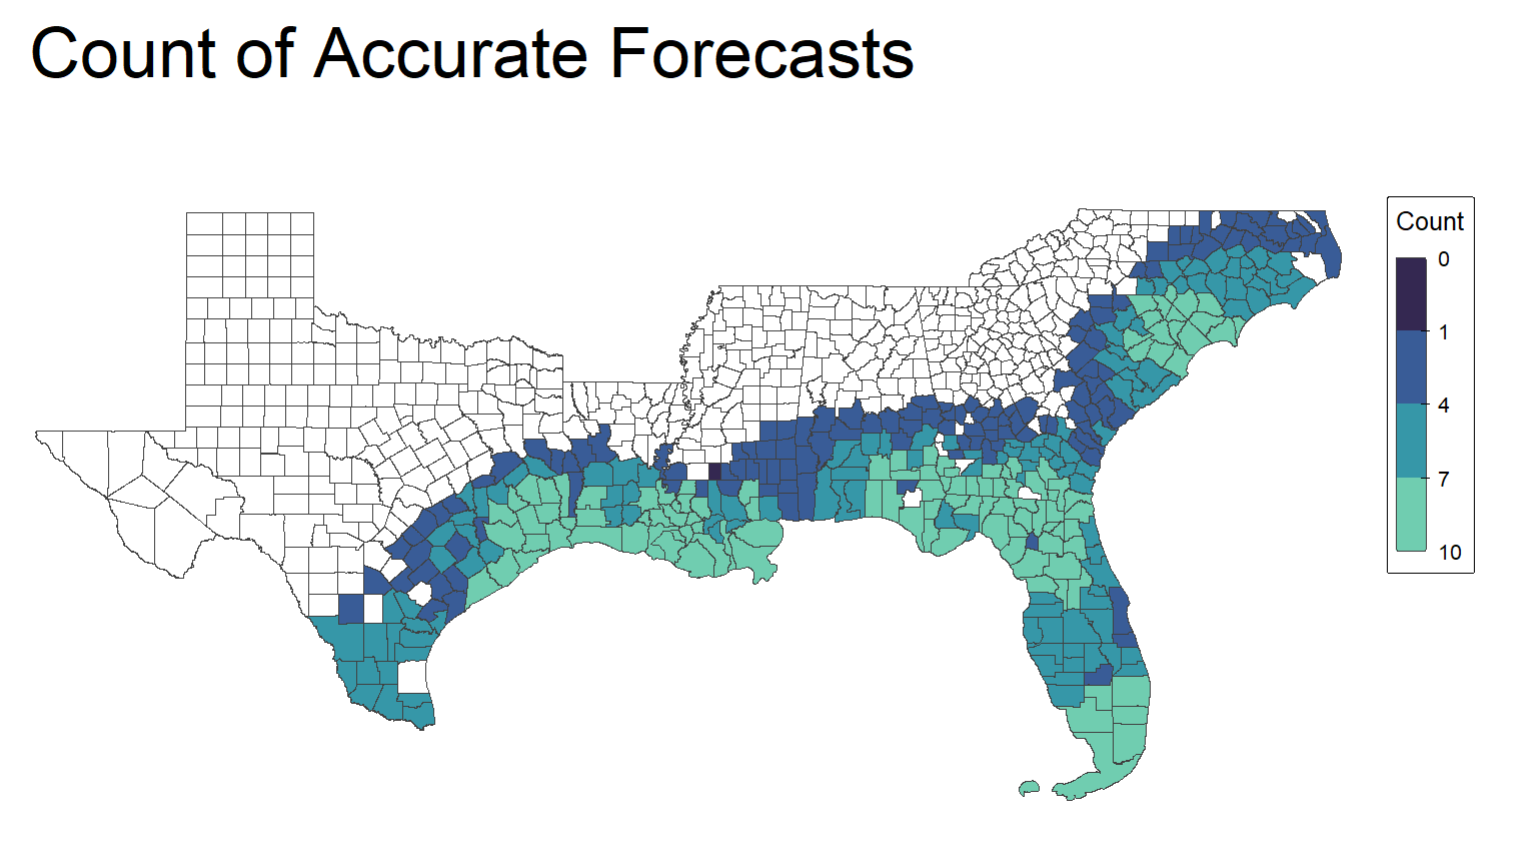
\includegraphics[width=0.65\linewidth]{True FC.png}
    \caption{Accurate Forecasts from 2008-2019}
    \label{fig:Hit FC}
    \floatfoot{Note: Map of all forecasts resulting in a hurricane landfall from 2008 to 2019. Darker counties had more accurate forecasts than lighter counties. Only counties with at least one landfall are colored.}
\end{figure}


\begin{figure}[!t]
    \centering
    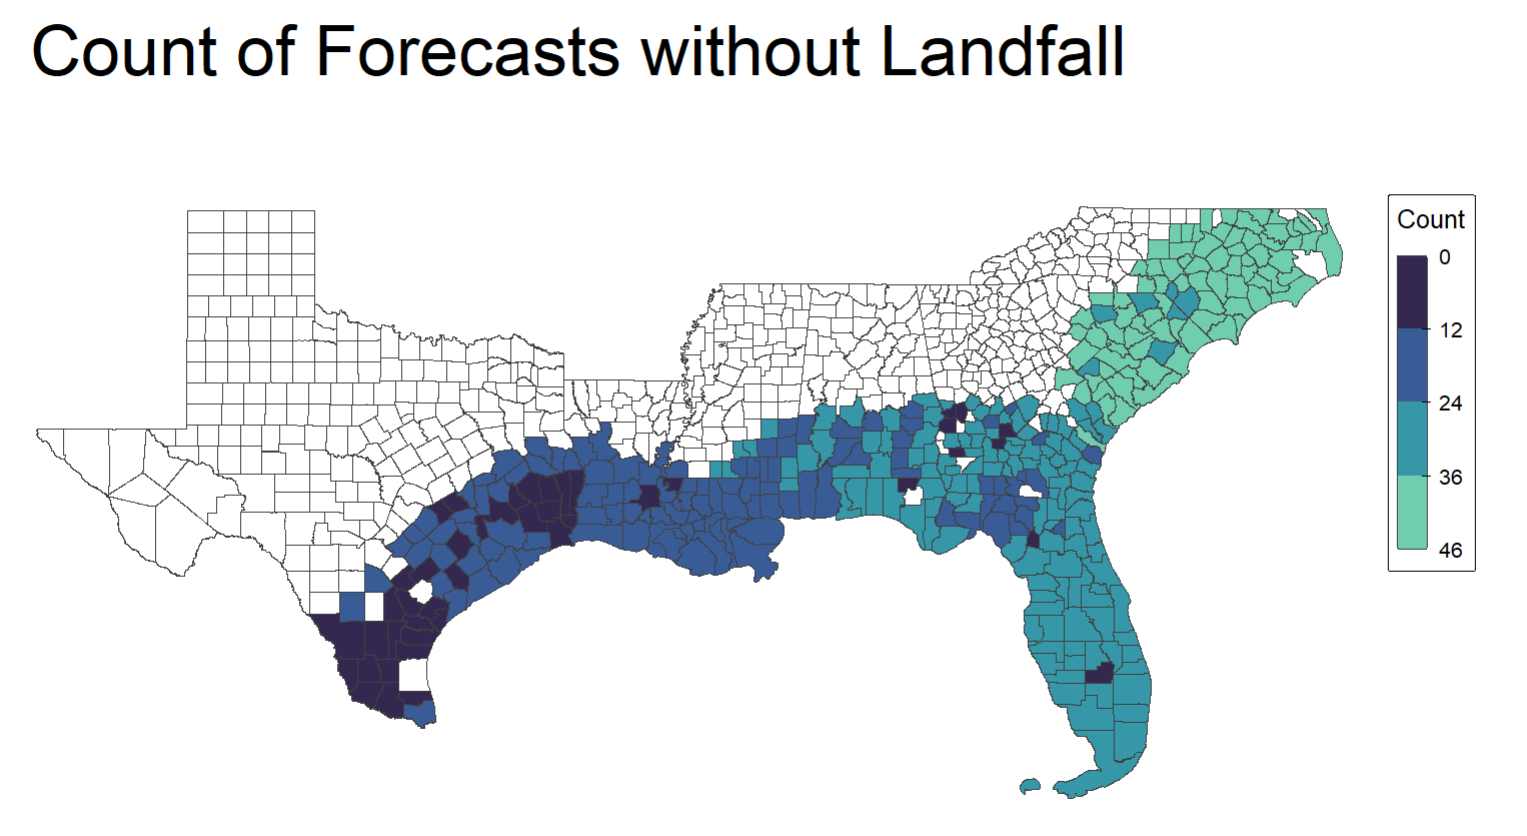
\includegraphics[width=0.65\linewidth]{Forecast no Land.png}
    \caption{Inaccurate Forecasts from 2008-2019}
    \label{fig:Miss FC}
    \floatfoot{Note: Map of all forecasts which did not result in a hurricane landfall from 2008 to 2019. Darker counties had more inaccurate forecasts than lighter counties. Only counties with at least one landfall are colored.}
\end{figure}

Figure \ref{fig:Hit FC} shows the total count of forecasts in each county that resulted in a Hurricane Landfall. This map suggests there may be some spacial correlation between counties that are often hit. Similarly, figure \ref{fig:Miss FC} shows the total count of forecasts that did not result in a landfall for each county. This map also suggests some level of spatial correlation. However, the maps are not inverses of one another, so there is still some variation when only looking at the effect of the most recent forecast result.




\begin{figure}[!t]
    \centering
    \begin{subfigure}{0.7\linewidth}
        \includegraphics[width=\linewidth]{2008 streak.png}
        %\caption{End of 2008}
    \end{subfigure}
    \begin{subfigure}{0.7\linewidth}
        \includegraphics[width=\linewidth]{2013 streak.png}
      % \caption{End of 2013}
    \end{subfigure}
    \caption{Streak of Forecast Accuracy}
    \label{fig:streak}
        \floatfoot{Note: Counties are colored by their accuracy streak at the end of the year. Counties in blue have had a streak of accurate forecasts and those in red have had streaks of inaccurate forecasts}
\end{figure}

 To determine if the hot-hand fallacy is at play, I create variables to indicate the streaks of the hit and miss forecasts. I build three versions of this variable for robustness. One is a pure hot-hand variable which increases by one for each hit forecast, but resets to zero whenever a miss occurs. The second definition is for a string of misses which increases by one for each miss and resets to zero when there is a hit. The third definition combines the previous two as an overall indicator of accuracy. At a first hit the streak is set to 1 and increases by 1 for each subsequent hit. At a first miss the variable is set to -1 and decreases by 1 for each subsequent miss. 
 
 Figure \ref{fig:streak} shows the accuracy streak fore each county at the end of 2008 and 2013. While the maps of total hits and misses in figures \ref{fig:Hit FC} and \ref{fig:Miss FC} show that certain areas are more or less prone to a certain result. Figure \ref{fig:streak} shows the streaks of the same result can vary drastically within a few years. 

\subsection{Control Data}

In addition to the scanner and forecast data above, I also utilize population and weather data for control. I use county level population reports from the \citeauthor{USCB}'s 2010 National Census. I utilize this data to scale the total revenue by each counties population. This keeps the larger coastal towns, like Miami and Houston, from driving the results. Because there may also be a tendency for people to purchase more bottled water in the warmer month when spending more time outdoors, I control for the mean temperature for each county-week observation. This data comes from \citeauthor{GHCN}'s Global Historical Daily Climatology Network. This data is aggregated to the weekly level by taking the mean of all reported daily mean temperatures for the given county-week. 

\section{Methodology}

\subsection{Recency Bias}

To determine if there is any recency bias, I estimate the effect of the last forecast and result for each county. I use a difference in differences model of the following specifications to obtain my results.

\begin{equation}
    \begin{split}
       Sales_{ct} = &\beta_1 Forecast_{ct} + \beta_2 Landfall_{ct} +\\ 
			&\beta_3 Forecast \times Prior Hit_{ct} + \beta_4 Landfall \times Prior Hit_{ct} + \\
			&\beta_5 Forecast \times Prior Miss_{ct} + \beta_6 Landfall \times Prior Miss_{ct} + \\
			& \alpha_c + \alpha_m + \alpha_y + \gamma X_{ct} + \varepsilon_{ct}\\
			\label{eq:rec}
    \end{split}
\end{equation}

In the model $Sales_{ct}$ is the log total revenue per 100 thousand residents for a county-week observation where the revenue comes from the NielsenIQ scanner data and the county population comes from the 2010 census. $Forecast$ indicates if a county boundary overlapped with a hurricane forecast during the week, and $Landfall$ indicates if the county was within the hurricanes radius upon landfall. $Prior Hit$ indicates if the last forecast the county saw resulted in a landfall; whereas, $Prior Miss$ indicates those last forecasts that did not result in a landfall. County, month, and year fixed effects are represented by $\alpha_c$, $\alpha_m$, and $\alpha_y$ respectively. $X$ is the control for mean temperature and $\varepsilon_ct$ is the errors. 

The primary coefficients of interest in the model are $\beta_3$, $\beta_4$, $\beta_5$, and $\beta_6$.  Any significance on the coefficient indicate that on average people learn from their most recent experiences. If $\beta_3 = \beta_5$ and $\beta_4 = \beta_6$ then the model implies that people learn from the exposure of hurricanes in general regardless of the outcome. If these results are not equal, then the model implies that people respond differently depending on how accurate forecasts are. In an ideal environment, the coefficient would be statistically the same, or even insignificant altogether. During hurricane season, sources such as the National Weather Service provide many services to help people learn about hurricanes and how to prepare for disasters. If people fully follow this information, then the outcome of the current storm should not change the way people prepare in the future. 

\subsection{Hot-Hand Fallacy}

If there are signs of recency bias, it is also possible that strings of inaccurate forecasts could further amplify such biases. In the gambling literature the hot-hand fallacy occurs whenever individuals believe that a streak of outcomes indicates a series even if the draws are independent from one another. In a similar but reverse manner, each hurricane forecast is independent, and is based on many current weather conditions surrounding the hurricane. It is possible that people still fall into a ``hot''-hand fallacy of sorts when there is a streak of forecasts that result in no hurricane landfall leading people to believe that the next forecast must also be wrong.  To test for this I use the following model. 

\begin{equation}
    \begin{split}
       Sales_{ct} = &\beta_1 Forecast_{ct} + \beta_2 Landfall_{ct} +\\ 
			&\beta_3 Forecast \times Streak_{ct} + \beta_4 Landfall \times Streak_{ct} + \\
			&\beta_5 Forecast \times Streak^2_{ct} + \beta_6 Landfall \times Streak^2_{ct} + \\
			& \alpha_c + \alpha_m + \alpha_y + \gamma X_{ct} + \varepsilon_{ct}\\
			\label{eq:hot}
    \end{split}
\end{equation}

Similar to equation(\ref{eq:rec}) $Sales_{ct}$ represents log total revenue per 100 thousand residents, $Forecast$ indicates overlap with a hurricane forecast, and $Landfall$ indicates overlap with a hurricane landfall.  County, month, and year fixed effects are represented by $\alpha_c$, $\alpha_m$, and $\alpha_y$ respectively. $X$ controls for mean weekly temperatures, and $\varepsilon_{ct}$ and errors. The variable $Streak_{ct}$ represents the current streak length of accurate or inaccurate forecasts. If individuals are falling into the how hand fallacy, longer streaks should further cement their beliefs and likewise affect their pattern of emergency supply purchases. Thus, $Streak$ enters into the equation quadratically. 

Parameter estimates $\beta_5$ and $\beta_6$ are the key parameters of interest for the hot-hand fallacy. While $\beta_3$ and $\beta_4$ help to reaffirm any findings for recency bias. A fallacy in beliefs occurs in the population when there is an over inference of the effect a streak has on potential outcomes. Thus, if either $\beta_5$ or $\beta_6$ is negative, then there is evidence of fallacy beliefs.

\section{Results}
\subsection{Preliminary Results}

I begin my analysis by estimating the effects of a current hurricane forecast and landfall on sales with a simplified version of the previous models:
\begin{equation}
    \begin{split}
       Sales_{ct} = &\beta_1 Forecast_{ct} + \beta_2 Landfall_{ct} +\\ 
			& \alpha_c + \alpha_m + \alpha_y + \gamma X_{ct} + \varepsilon_{ct}\\
			\label{eq:simple}
    \end{split}
\end{equation}
The variables are defined the same as in equations (\ref{eq:rec}) and (\ref{eq:hot}). Because hurricanes are forecast up to five days out, I test multiple definition of the $Forecast$ variable. First I use the definition from above, if at any point a county overlaps with the forecast path of the hurricane. I then break this definition up by days until landfall. When a county if in the path of a future hurricane they can be 4 or 5 days from potential landfall which is called and \emph{Early Forecast}. If the county is 3 days from a potential landfall then they are in the \emph{Middle Forecast}. Counties which are 1 to 2 days from a potential landfall have a \emph{Late Forecast}. During a given hurricane counties can be in any combination of the different forecast categories.

\begin{table}[!t]
   \caption{Effect of Current Forecast on Sales}
   \centering
   \begin{tabular}{lccccc}
      \tabularnewline \midrule \midrule
      Dependent Variable: & \multicolumn{5}{c}{Sales}\\
      Model:       & (1)            & (2)            & (3)            & (4)            & (5)\\  
      \midrule
      \emph{Variables}\\
      Any Forecast        & 0.0401$^{***}$ &                &                &                &   \\   
                   & (0.0043)       &                &                &                &   \\   

      Early Forecast      &                & 0.0481$^{***}$ &                &                & 0.0458$^{***}$\\   
                   &                & (0.0044)       &                &                & (0.0050)\\   
      Middle Forecast        &                &                & 0.0411$^{***}$ &                & 0.0246$^{***}$\\   
                   &                &                & (0.0071)       &                & (0.0093)\\   
      Late Forecast       &                &                &                & 0.0120         & -0.0336$^{***}$\\   
                   &                &                &                & (0.0086)       & (0.0103)\\   
                   
      Landfall     & 0.1962$^{***}$ & 0.2079$^{***}$ & 0.2037$^{***}$ & 0.2192$^{***}$ & 0.2233$^{***}$\\   
                   & (0.0199)       & (0.0194)       & (0.0199)       & (0.0207)       & (0.0206)\\   
      \midrule
      \emph{Fit statistics}\\
      Observations & 448,123        & 448,123        & 448,123        & 448,123        & 448,123\\  
      R$^2$        & 0.77052        & 0.77053        & 0.77051        & 0.77048        & 0.77054\\  
      \midrule \midrule
        \floatfoot{Results from the regression in equation (\ref{eq:simple}).  Clustered (county) standard-errors are in parentheses. Sales is the log total revenue per 100 thousand residents in U.S. dollars at the county-week level. Signif. Codes:  ***: 0.01, **: 0.05, *: 0.1 }
   \end{tabular}
   \label{tab:simple}
\end{table}

Results of equation (\ref{eq:simple}) and the different definitions of a forecast can be found in table \ref{tab:simple}.  Column (1) shows that for any hurricane forecast, county level sales of bottled water increase by just over 4\%,  whereas a landfall increases sales by just over 12\%. The early and middle forecasts also see significant increases in sale. The late forecast does not show significant increases in sales; however, the estimate on landfall has increased to absorb the increase. Since there is less time until landfall in the late category, there are more observances of the late forecast and landfall weeks overlapping perfectly explaining this change in estimates. Similar results are found in column (5) when the three timing forecast variables are included at once. Due to the potential strong collinearity with the late forecast variable, I elect to focus on the inclusive variable, any forecast, for the remainder of the analysis. Results for the other definitions of forecast are included in the appendix. 

\subsection{Recency Bias Results}


\begin{table}[htbp]
   \caption{Effect of Most Recent Forecast Outcome}
   \centering
   \begin{tabular}{lcccc}
      \tabularnewline \midrule \midrule
      Dependent Variable: & \multicolumn{4}{c}{log(total\_rev\_per\_cap)}\\
      Model:                                  & (1)            & (2)             & (3)             & (4)\\  
      \midrule
      \emph{Variables}\\
      anyTG                                   & 0.0401$^{***}$ & 0.0461$^{***}$  & 0.1128$^{***}$  & -0.3359$^{***}$\\   
                                              & (0.0043)       & (0.0043)        & (0.0182)        & (0.1268)\\   
      Landfall                                & 0.1962$^{***}$ & 0.2723$^{***}$  & 0.0764$^{**}$   & 1.307$^{***}$\\   
                                              & (0.0199)       & (0.0271)        & (0.0387)        & (0.4178)\\   
      temp\_mean                              & 0.0046$^{***}$ & 0.0046$^{***}$  & 0.0046$^{***}$  & 0.0046$^{***}$\\   
                                              & (0.0004)       & (0.0004)        & (0.0004)        & (0.0004)\\   
      anyTG $\times$ last\_anyTG\_Hit         &                & 0.0890$^{***}$  &                 & 0.4709$^{***}$\\   
                                              &                & (0.0190)        &                 & (0.1271)\\   
      Landfall $\times$ last\_anyTG\_Hit      &                & -0.2272$^{***}$ &                 & -1.262$^{***}$\\   
                                              &                & (0.0524)        &                 & (0.4203)\\   
      anyTG $\times$ last\_anyTG\_NoHit       &                &                 & -0.0654$^{***}$ & 0.3833$^{***}$\\   
                                              &                &                 & (0.0195)        & (0.1273)\\   
      Landfall $\times$ last\_anyTG\_NoHit    &                &                 & 0.1888$^{***}$  & -1.042$^{**}$\\   
                                              &                &                 & (0.0533)        & (0.4187)\\   
      \midrule
      \emph{Fixed-effects}\\
      fips                                    & Yes            & Yes             & Yes             & Yes\\  
      month                                   & Yes            & Yes             & Yes             & Yes\\  
      year                                    & Yes            & Yes             & Yes             & Yes\\  
      \midrule
      \emph{Fit statistics}\\
      Observations                            & 448,123        & 419,543         & 419,543         & 419,543\\  
      R$^2$                                   & 0.77052        & 0.76552         & 0.76551         & 0.76554\\  
      \midrule \midrule
      \multicolumn{5}{l}{\emph{Clustered (fips) standard-errors in parentheses}}\\
      \multicolumn{5}{l}{\emph{Signif. Codes: ***: 0.01, **: 0.05, *: 0.1}}\\
   \end{tabular}
\end{table}


Tests for recency bias follow the model from equation (\ref{eq:rec}) and can be found in table \ref{tab:rec}. Column (1) repeats the main findings from the simplified regression results in table \ref{tab:simple}. Once variables for prior forecast results are added to the model, the sign on forecast flips, with the prior outcomes determining the magnitude of purchases. The effect of a hurricane landfall is still positive and significantly larger, with the prior result determining the final magnitude of sales. Using the results from column (4) the estimated increase in sales from a current hurricane forecast is roughly 4.3\% when the the last hurricane hit and 6.0\% when the last hurricane missed. Similarly, the estimated increase in sales from a current landfall is 3.4\% when the last hurricane hit and 21.2\% when the last hurricane missed. 

While the estimates in table \ref{tab:rec} are significant, they do not show evidence of recency bias unless they are also statistically different from one another. Specifically, the following hypothesis test must be rejected:

\begin{equation*}
\begin{split}
H_0: \beta_3 = \beta_5 and \beta_4 = \beta_6 \\
H_1: \beta_3 \neq \beta_5 or \beta_4 \neq \beta_6
\end{split}
\end{equation*}

To test this hypothesis, I modify the model from equation (\ref{eq:rec}) in the following manner:
\begin{equation}
    \begin{split}
       Sales_{ct} = &\beta_1 Forecast_{ct} + \beta_2 Landfall_{ct} +\\ 
			&\beta_3 \left( Forecast \times Prior Hit_{ct} + Forecast \times Prior Miss_{ct} \right)  + \\
			& \beta_4 \left(  Landfall \times Prior Hit_{ct} + Landfall \times Prior Miss_{ct} \right) + \\
			& \alpha_c + \alpha_m + \alpha_y + \gamma X_{ct} + \varepsilon_{ct}\\
			\label{eq:ftest}
    \end{split}
\end{equation}



\begin{table}[!t]
   \caption{Test for Recency Bias}
   \centering
   \begin{tabular}{lccc}
      \tabularnewline \midrule \midrule
       & (1) & (2) & (3)\\
      Test Criteria: & $\beta_3 = \beta_5$ & $\beta_4 = \beta_6$ & $\beta_3 = \beta_5 \& \beta_4 = \beta_6$\\
      \midrule
      \emph{Test Statistic}\\
      $\chi^2$      &21.276 &  17.751   &  29.367            \\   
     
          &   ($3.9\times 10^{-6}$)    & ($2.5\times 10^{-5}$)  &  ($4.2\times 10^{-7}$)     \\   

      \midrule \midrule
        \floatfoot{Result of F-test using the test criteria as the restricted model and equation (\ref{eq:rec}) as the unrestricted model.  p-values are reported parentheses. Sales is the log total revenue per 100 thousand residents in U.S. dollars at the county-week level. Signif. Codes:  ***: 0.01, **: 0.05, *: 0.1 }
   \end{tabular}
   \label{tab:ftest}
\end{table}

The results from this test are found in table \ref{tab:ftest}. Column (1) shows the result of testing for differences in only the forecast variables. Under this weaker test, there is not enough evidence to determine recency bias in the population decision to purchase emergency supplies. Columns (2) and (3), which test for difference in the landfall variables and the combined test of forecast and landfall variables, have significantly low p-values. Overall, this suggests that there is strong evidence of recency bias, with the larger effect of the bias occurring later in the forecast cycle when a landfall is more assured. 

As a robustness test, I rerun the prior regressions and F-test using the different definitions of forecast based on timing. This ensures that the bias is consistent across all points of the hurricane forecast, and not just based on the way the forecasts land in the weekly level data. Table \ref{tab:rec_app} of the appendix shows the regression results for the different timing of the forecast. Under all definitions the effect of the most recent forecast is significant. The results of the F-tests are shown in table \ref{tab:ftest_app} of the appendix, which further demonstrates that recency bias is prevalent no matter how we cut the hurricane forecast. 

\subsection{Hot Hand Results}

\begin{table}[htbp]
   \caption{Effect of Streaks of Forecast Outcomes}
   \centering
   \begin{tabular}{lcccccc}
      \tabularnewline \midrule \midrule
      Dependent Variable: & \multicolumn{6}{c}{log(total\_rev\_per\_cap)}\\
       & \multicolumn{2}{c}{Hit} & \multicolumn{2}{c}{Miss} & \multicolumn{2}{c}{Accuracy} \\ 
      Model:                  & (1)             & (2)             & (3)             & (4)             & (5)            & (6)\\  
      \midrule
      \emph{Variables}\\
      anyTG                   & 0.0470$^{***}$  & 0.0463$^{***}$  & 0.1003$^{***}$  & 0.0870$^{***}$  & 0.1551$^{***}$ & 0.1640$^{***}$\\   
                              & (0.0042)        & (0.0043)        & (0.0105)        & (0.0107)        & (0.0126)       & (0.0129)\\   
      Landfall                & 0.3134$^{***}$  & 0.2814$^{***}$  & 0.1225$^{***}$  & 0.0950$^{***}$  & 0.1552$^{***}$ & 0.1830$^{***}$\\   
                              & (0.0247)        & (0.0267)        & (0.0256)        & (0.0306)        & (0.0331)       & (0.0318)\\   
      anyTG\_hit              & 0.0510$^{***}$  & 0.0918$^{***}$  &                 &                 &                &   \\   
                              & (0.0097)        & (0.0295)        &                 &                 &                &   \\   
      land\_hit               & -0.2474$^{***}$ & -0.0355         &                 &                 &                &   \\   
                              & (0.0381)        & (0.0775)        &                 &                 &                &   \\   
      anyTG\_hit\_sq          &                 & -0.0185         &                 &                 &                &   \\   
                              &                 & (0.0117)        &                 &                 &                &   \\   
      land\_hit\_sq           &                 & -0.1131$^{***}$ &                 &                 &                &   \\   
                              &                 & (0.0321)        &                 &                 &                &   \\   
      anyTG\_miss             &                 &                 & -0.0050$^{***}$ & -0.0015         &                &   \\   
                              &                 &                 & (0.0012)        & (0.0027)        &                &   \\   
      land\_miss              &                 &                 & 0.0153$^{***}$  & 0.0409$^{***}$  &                &   \\   
                              &                 &                 & (0.0042)        & (0.0109)        &                &   \\   
      anyTG\_miss\_sq         &                 &                 &                 & -0.0001         &                &   \\   
                              &                 &                 &                 & (0.0001)        &                &   \\   
      land\_miss\_sq          &                 &                 &                 & -0.0015$^{***}$ &                &   \\   
                              &                 &                 &                 & (0.0006)        &                &   \\   
      anyTG\_acc\_cont        &                 &                 &                 &                 & 0.0081$^{***}$ & 0.0099$^{***}$\\   
                              &                 &                 &                 &                 & (0.0011)       & (0.0016)\\   
      land\_acc\_cont         &                 &                 &                 &                 & -0.0031        & 0.0064\\   
                              &                 &                 &                 &                 & (0.0037)       & (0.0041)\\   
      anyTG\_acc\_cont\_sq    &                 &                 &                 &                 &                & $8.12\times 10^{-5}$\\    
                              &                 &                 &                 &                 &                & ($6.35\times 10^{-5}$)\\    
      land\_acc\_cont\_sq     &                 &                 &                 &                 &                & 0.0012$^{***}$\\   
                              &                 &                 &                 &                 &                & (0.0002)\\   
      \midrule
      \emph{Fixed-effects}\\
      fips                    & Yes             & Yes             & Yes             & Yes             & Yes            & Yes\\  
      month                   & Yes             & Yes             & Yes             & Yes             & Yes            & Yes\\  
      year                    & Yes             & Yes             & Yes             & Yes             & Yes            & Yes\\  
      \midrule
      \emph{Fit statistics}\\
      Observations            & 419,537         & 419,537         & 419,537         & 419,537         & 419,537        & 419,537\\  
      R$^2$                   & 0.76555         & 0.76557         & 0.76556         & 0.76557         & 0.76566        & 0.76570\\  
      \midrule \midrule
      \multicolumn{7}{l}{\emph{Clustered (fips) standard-errors in parentheses}}\\
      \multicolumn{7}{l}{\emph{Signif. Codes: ***: 0.01, **: 0.05, *: 0.1}}\\
   \end{tabular}
\end{table}


To test for evidence of the hot-hand fallacy, I use equation (\ref{eq:hot}) along with different definitions of a streak. The results for all definitions can be found in table \ref{tab:hot}. A hot-hand in the traditional sense would come from a string of accurate weather forecasts leading the population to believe that the forecasts can never be wrong. The coefficients under this more traditional definition are found in column (2). While only the estimate of $Landfall \times Streak^2$ is significant, it still indicates some level of hot-hand beliefs. The estimates indicate that any amount of consecutive correct forecasts leads to significant reductions in panic buying of emergency supplies. 

While streaks of current forecasts lead to some hot-hand behavior, streaks of incorrect forecasts happen much more frequently and tend to last longer. To test if the hot-hand fallacy holds for string of negative results, I look to column (4) of table \ref{tab:hot}.
With significant negative estimates on both squared terms, there is strong evidence to suggest that the hot-hand fallacy can also hold for strings of negative outcomes. Specifically, these parameters imply that as streaks of incorrect forecasts lengthen, panic buying becomes increasingly worse once an accurate forecast is finally realized. 

As a robustness check, I also use a definition that includes both streaks of hits and misses with hits being represented positively and misses negatively. The results from this definition can be found in columns (5) and (6).  This definition returns parameters that are quite similar to those in columns (3) and (4). The resulting interpretation is the same. Streaks of more accurate forecasts will result in less panic buying, and streaks of inaccurate forecasts will increase panic buying once a hurricane finally makes landfall. 



\subsection{Implication of Results}

The increased panic buying coming from recency bias and the hot-hand fallacy impacts states with more misses than hits. Historically, the states most prone to inaccurate forecasts are those of the South Atlantic Coast, namely North Carolina, South Carolina, Georgia, and Florida. Thus, these states will likely benefit the most from improved forecasting methods and technology. The results in table \ref{tab:hot} imply that panic buying will begin to decrease if the number of consecutive inaccurate forecasts remains less than 16. I use this metric to simulate a world with better forecasting technology. To build this data, I begin by calculating the streaks of misses and hits as in the data section. For this data, I set a hard rule that the 16th forecast must result in a landfall. 


\begin{figure}[!t]
    \centering
    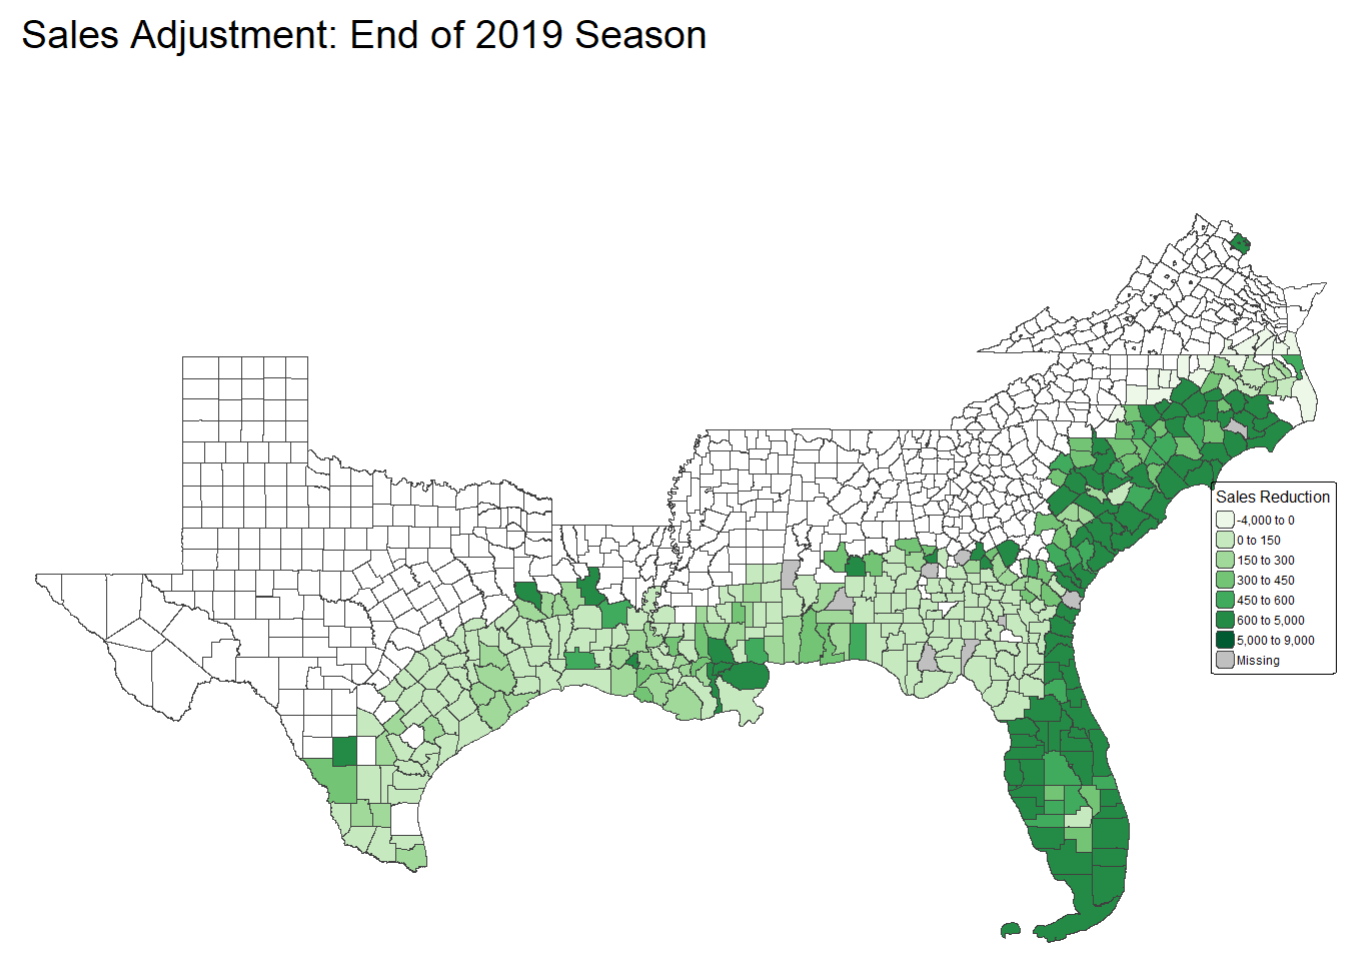
\includegraphics[width=0.65\linewidth]{Sales dif 2019.png}
    \caption{Estimated Reduction in Panic Buying}
    \label{fig:simulation}
    \floatfoot{Note: Map of the estimated reduction in emergency supply sales the week of a hurricane landfall at the end of the 2019 hurricane season. Sales is total revenue per 100 thousand residents in USD.  Darker counties benefit the most from reduced panic buying with more accurate forecasts. Only counties with at least one landfall from 2008-2019 are colored.}
\end{figure}

To determine the difference in sales of emergency supplies resulting from a hurricane forecast and landfall, I assume that a hurricane hits all counties on the last day of hurricane season in 2019 (November 30th). Using the results from column (6) of table \ref{tab:hot} I estimate the total revenue per 100 thousand residents for each county under both the original data, and the simulated better forecast data. Figure \ref{fig:simulation} shows the predicted change in sales for all counties. The largest effect is on the Atlantic coast as predicted. Reductions in these four most effected states are on average over \$75 per 100 thousand residents and as large as nearly \$3,000 per 100 thousand residents. One thing to notice is that some counties show an increase in sales around a hurricane. These counties all have 30 or more misses in a row. The model suggests that the people in these counties have such strong beliefs that the hurricane will miss that they currently respond much less to forecasts than other counties. Such places beginning to see accurate forecasts would, at first, increase their panic buying before over time reducing it. 

\section{Conclusion}

There is strong evidence that the population on average waits until the last minute to purchase emergency supplies for hurricanes. However, there is less know about the factors that affect the magnitude of these purchases. The decision of how much to prepare for an impending natural disaster could be thought of as the determination of anticipated risk from the disaster. Because of this I look to the risk and gambling literature for an explanation in variation in emergency supply sales from one disaster to the next. 

Using results from past hurricane forecasts and sales of bottled water, I test for both recency bias and hot-hand bias. I find significant evidence of recency bias with the last forecast resulting in no landfall leading to significantly higher sales than when the last forecast was accurate. Additionally, I find significant evidence of the hot-hand fallacy which follows results from experimental and gambling literature. Specifically, sales increase as forecasts become less and less accurate; however, once there are more than 15 inaccurate forecasts in a row the response begins to reduce. Through estimating a better forecast timeline I find that as technology for forecasts improves, panic buying will likely reduce significantly, and by over \$4,000 per 100 thousand residents along some parts of the East Coast. 

\newpage
 \bibliographystyle{apalike}
 \bibliography{biblio}
\newpage



\begin{appendices}
\section*{Appendix}
\setcounter{table}{0}
\renewcommand{\thetable}{A\arabic{table}}


\begin{table}[htbp]
   \caption{Effect of Most Recent Forecast Outcome}
   \centering
   \begin{tabular}{lcccc}
      \tabularnewline \midrule \midrule
      Dependent Variable: & \multicolumn{4}{c}{log(total\_rev\_per\_cap)}\\
                                              & Any             & Early           & Middle          & Late \\   
      Model:                                  & (1)             & (2)             & (3)             & (4)\\  
      \midrule
      \emph{Variables}\\
      anyTG                                   & -0.3359$^{***}$ &                 &                 &   \\   
                                              & (0.1268)        &                 &                 &   \\   
      Landfall                                & 1.307$^{***}$   & 0.9710$^{**}$   & 1.426$^{***}$   & 1.673$^{***}$\\   
                                              & (0.4178)        & (0.3839)        & (0.4862)        & (0.4131)\\   
      temp\_mean                              & 0.0046$^{***}$  & 0.0046$^{***}$  & 0.0046$^{***}$  & 0.0046$^{***}$\\   
                                              & (0.0004)        & (0.0004)        & (0.0004)        & (0.0004)\\   
      anyTG $\times$ last\_anyTG\_Hit         & 0.4709$^{***}$  &                 &                 &   \\   
                                              & (0.1271)        &                 &                 &   \\   
      Landfall $\times$ last\_anyTG\_Hit      & -1.262$^{***}$  & -0.8822$^{**}$  & -1.428$^{***}$  & -1.726$^{***}$\\   
                                              & (0.4203)        & (0.3908)        & (0.4897)        & (0.4162)\\   
      anyTG $\times$ last\_anyTG\_NoHit       & 0.3833$^{***}$  &                 &                 &   \\   
                                              & (0.1273)        &                 &                 &   \\   
      Landfall $\times$ last\_anyTG\_NoHit    & -1.042$^{**}$   & -0.6916$^{*}$   & -1.148$^{**}$   & -1.382$^{***}$\\   
                                              & (0.4187)        & (0.3836)        & (0.4867)        & (0.4150)\\   
      earlyTG                                 &                 & -0.3462$^{***}$ &                 &   \\   
                                              &                 & (0.1287)        &                 &   \\   
      earlyTG $\times$ last\_anyTG\_Hit       &                 & 0.4919$^{***}$  &                 &   \\   
                                              &                 & (0.1307)        &                 &   \\   
      earlyTG $\times$ last\_anyTG\_NoHit     &                 & 0.4028$^{***}$  &                 &   \\   
                                              &                 & (0.1292)        &                 &   \\   
      midTG                                   &                 &                 & -0.5345$^{***}$ &   \\   
                                              &                 &                 & (0.1567)        &   \\   
      midTG $\times$ last\_anyTG\_Hit         &                 &                 & 0.7600$^{***}$  &   \\   
                                              &                 &                 & (0.1595)        &   \\   
      midTG $\times$ last\_anyTG\_NoHit       &                 &                 & 0.5795$^{***}$  &   \\   
                                              &                 &                 & (0.1573)        &   \\   
      lateTG                                  &                 &                 &                 & -0.7064$^{***}$\\   
                                              &                 &                 &                 & (0.1508)\\   
      lateTG $\times$ last\_anyTG\_Hit        &                 &                 &                 & 0.9373$^{***}$\\   
                                              &                 &                 &                 & (0.1537)\\   
      lateTG $\times$ last\_anyTG\_NoHit      &                 &                 &                 & 0.7214$^{***}$\\   
                                              &                 &                 &                 & (0.1521)\\   
      \midrule
      \emph{Fixed-effects}\\
      fips                                    & Yes             & Yes             & Yes             & Yes\\  
      month                                   & Yes             & Yes             & Yes             & Yes\\  
      year                                    & Yes             & Yes             & Yes             & Yes\\  
      \midrule
      \emph{Fit statistics}\\
      Observations                            & 419,543         & 419,543         & 419,543         & 419,543\\  
      R$^2$                                   & 0.76554         & 0.76555         & 0.76554         & 0.76551\\  
      \midrule \midrule
      \multicolumn{5}{l}{\emph{Clustered (fips) standard-errors in parentheses}}\\
      \multicolumn{5}{l}{\emph{Signif. Codes: ***: 0.01, **: 0.05, *: 0.1}}\\
   \end{tabular}
\end{table}



\begin{table}[htbp]
   \caption{Tests for Recency Bias}
   \centering
   \begin{tabular}{lcccc}
      \tabularnewline \midrule \midrule
       & (1) & (2) & (3) & (4)\\
      Forecast Type: & Any & Early & Middle & Late\\
      \midrule
      \emph{Test Statistic}\\
      $\chi^2$     & 29.367 &    28.23    & 57.046& 29.367    \\   
         	 &  (4.2$\times 10^{-7}$) &  (7.4$\times 10^{-7}$)  & (4.1$\times 10^{-13}$)  & (4.2$\times 10^{-7}$) \\   

      \midrule \midrule
        \floatfoot{Result of F-test using the test criteria as the restricted model and equation (\ref{eq:rec}) as the unrestricted model.  p-values are reported parentheses. Sales is the log total revenue per 100 thousand residents in U.S. dollars at the county-week level. Signif. Codes:  ***: 0.01, **: 0.05, *: 0.1 }
   \end{tabular}
   \label{tab:ftest_app}
\end{table}


\begin{table}[htbp]
   \caption{Effect of Streaks of Forecast Outcomes}
   \centering
   \begin{tabular}{lcccc}
      \tabularnewline \midrule \midrule
      Dependent Variable: & \multicolumn{4}{c}{log(total\_rev\_per\_cap)}\\
      Model:            & (1)             & (2)             & (3)             & (4)\\  
      \midrule
      \emph{Variables}\\
      anyTG             & 0.0996$^{***}$  & 0.0893$^{***}$  & 0.0946$^{***}$  & 0.0707$^{***}$\\   
                        & (0.0101)        & (0.0095)        & (0.0121)        & (0.0132)\\   
      Landfall          & 0.1238$^{***}$  & 0.1178$^{***}$  & 0.2890$^{***}$  & 0.1676$^{***}$\\   
                        & (0.0245)        & (0.0246)        & (0.0390)        & (0.0569)\\   
      anyTG\_acc        & 0.0050$^{***}$  & 0.0021          &                 &   \\   
                        & (0.0011)        & (0.0025)        &                 &   \\   
      land\_acc         & -0.0167$^{***}$ & -0.0420$^{***}$ &                 &   \\   
                        & (0.0040)        & (0.0095)        &                 &   \\   
      temp\_mean        & 0.0046$^{***}$  & 0.0046$^{***}$  & 0.0046$^{***}$  & 0.0046$^{***}$\\   
                        & (0.0004)        & (0.0004)        & (0.0004)        & (0.0004)\\   
      anyTG\_acc\_sq    &                 & -0.0001         &                 &   \\   
                        &                 & (0.0001)        &                 &   \\   
      land\_acc\_sq     &                 & -0.0016$^{***}$ &                 &   \\   
                        &                 & (0.0005)        &                 &   \\   
      anyTG\_hit        &                 &                 & 0.0257$^{**}$   & 0.0657$^{**}$\\   
                        &                 &                 & (0.0120)        & (0.0315)\\   
      land\_hit         &                 &                 & -0.2371$^{***}$ & 0.1072\\   
                        &                 &                 & (0.0470)        & (0.1006)\\   
      anyTG\_miss       &                 &                 & -0.0047$^{***}$ & 0.0009\\   
                        &                 &                 & (0.0013)        & (0.0030)\\   
      land\_miss        &                 &                 & 0.0010          & 0.0263$^{*}$\\   
                        &                 &                 & (0.0051)        & (0.0141)\\   
      anyTG\_hit\_sq    &                 &                 &                 & -0.0124\\   
                        &                 &                 &                 & (0.0119)\\   
      land\_hit\_sq     &                 &                 &                 & -0.1495$^{***}$\\   
                        &                 &                 &                 & (0.0350)\\   
      anyTG\_miss\_sq   &                 &                 &                 & -0.0002$^{*}$\\   
                        &                 &                 &                 & (0.0001)\\   
      land\_miss\_sq    &                 &                 &                 & -0.0010\\   
                        &                 &                 &                 & (0.0006)\\   
      \midrule
      \emph{Fixed-effects}\\
      fips              & Yes             & Yes             & Yes             & Yes\\  
      month             & Yes             & Yes             & Yes             & Yes\\  
      year              & Yes             & Yes             & Yes             & Yes\\  
      \midrule
      \emph{Fit statistics}\\
      Observations      & 419,537         & 419,537         & 419,537         & 419,537\\  
      R$^2$             & 0.76556         & 0.76558         & 0.76560         & 0.76562\\  
      \midrule \midrule
      \multicolumn{5}{l}{\emph{Clustered (fips) standard-errors in parentheses}}\\
      \multicolumn{5}{l}{\emph{Signif. Codes: ***: 0.01, **: 0.05, *: 0.1}}\\
   \end{tabular}
\end{table}



\begin{table}[htbp]
   \caption{Effect of Streaks of Forecast Outcomes by Timing}
   \centering
   \begin{tabular}{lcccccccc}
      \tabularnewline \midrule \midrule
      Dependent Variable: & \multicolumn{8}{c}{log(total\_rev\_per\_cap)}\\
      Model:             & (1)             & (2)             & (3)             & (4)                    & (5)             & (6)             & (7)             & (8)\\  
      \midrule
      \emph{Variables}\\
      anyTG              & 0.0996$^{***}$  & 0.0893$^{***}$  &                 &                        &                 &                 &                 &   \\   
                         & (0.0101)        & (0.0095)        &                 &                        &                 &                 &                 &   \\   
      Landfall           & 0.1238$^{***}$  & 0.1178$^{***}$  & 0.1582$^{***}$  & 0.1447$^{***}$         & 0.1431$^{***}$  & 0.1133$^{***}$  & 0.1426$^{***}$  & 0.1150$^{***}$\\   
                         & (0.0245)        & (0.0246)        & (0.0231)        & (0.0237)               & (0.0233)        & (0.0242)        & (0.0244)        & (0.0256)\\   
      anyTG\_acc         & 0.0050$^{***}$  & 0.0021          &                 &                        &                 &                 &                 &   \\   
                         & (0.0011)        & (0.0025)        &                 &                        &                 &                 &                 &   \\   
      land\_acc          & -0.0167$^{***}$ & -0.0420$^{***}$ & -0.0148$^{***}$ & -0.0425$^{***}$        & -0.0155$^{***}$ & -0.0487$^{***}$ & -0.0167$^{***}$ & -0.0483$^{***}$\\   
                         & (0.0040)        & (0.0095)        & (0.0038)        & (0.0093)               & (0.0039)        & (0.0094)        & (0.0040)        & (0.0096)\\   
      temp\_mean         & 0.0046$^{***}$  & 0.0046$^{***}$  & 0.0046$^{***}$  & 0.0046$^{***}$         & 0.0046$^{***}$  & 0.0046$^{***}$  & 0.0046$^{***}$  & 0.0046$^{***}$\\   
                         & (0.0004)        & (0.0004)        & (0.0004)        & (0.0004)               & (0.0004)        & (0.0004)        & (0.0004)        & (0.0004)\\   
      anyTG\_acc\_sq     &                 & -0.0001         &                 &                        &                 &                 &                 &   \\   
                         &                 & (0.0001)        &                 &                        &                 &                 &                 &   \\   
      land\_acc\_sq      &                 & -0.0016$^{***}$ &                 & -0.0017$^{***}$        &                 & -0.0019$^{***}$ &                 & -0.0019$^{***}$\\   
                         &                 & (0.0005)        &                 & (0.0005)               &                 & (0.0005)        &                 & (0.0005)\\   
      earlyTG            &                 &                 & 0.1087$^{***}$  & 0.1045$^{***}$         &                 &                 &                 &   \\   
                         &                 &                 & (0.0105)        & (0.0096)               &                 &                 &                 &   \\   
      earlyTG\_acc       &                 &                 & 0.0050$^{***}$  & 0.0037                 &                 &                 &                 &   \\   
                         &                 &                 & (0.0012)        & (0.0025)               &                 &                 &                 &   \\   
      earlyTG\_acc\_sq   &                 &                 &                 & $-4.68\times 10^{-5}$  &                 &                 &                 &   \\   
                         &                 &                 &                 & (0.0001)               &                 &                 &                 &   \\   
      midTG              &                 &                 &                 &                        & 0.1030$^{***}$  & 0.1216$^{***}$  &                 &   \\   
                         &                 &                 &                 &                        & (0.0114)        & (0.0126)        &                 &   \\   
      midTG\_acc         &                 &                 &                 &                        & 0.0051$^{***}$  & 0.0105$^{***}$  &                 &   \\   
                         &                 &                 &                 &                        & (0.0013)        & (0.0029)        &                 &   \\   
      midTG\_acc\_sq     &                 &                 &                 &                        &                 & 0.0002$^{*}$    &                 &   \\   
                         &                 &                 &                 &                        &                 & (0.0001)        &                 &   \\   
      lateTG             &                 &                 &                 &                        &                 &                 & 0.0744$^{***}$  & 0.0866$^{***}$\\   
                         &                 &                 &                 &                        &                 &                 & (0.0121)        & (0.0154)\\   
      lateTG\_acc        &                 &                 &                 &                        &                 &                 & 0.0050$^{***}$  & 0.0083$^{**}$\\   
                         &                 &                 &                 &                        &                 &                 & (0.0013)        & (0.0033)\\   
      lateTG\_acc\_sq    &                 &                 &                 &                        &                 &                 &                 & 0.0001\\   
                         &                 &                 &                 &                        &                 &                 &                 & (0.0001)\\   
      \midrule
      \emph{Fixed-effects}\\
      fips               & Yes             & Yes             & Yes             & Yes                    & Yes             & Yes             & Yes             & Yes\\  
      month              & Yes             & Yes             & Yes             & Yes                    & Yes             & Yes             & Yes             & Yes\\  
      year               & Yes             & Yes             & Yes             & Yes                    & Yes             & Yes             & Yes             & Yes\\  
      \midrule
      \emph{Fit statistics}\\
      Observations       & 419,537         & 419,537         & 419,537         & 419,537                & 419,537         & 419,537         & 419,537         & 419,537\\  
      R$^2$              & 0.76556         & 0.76558         & 0.76557         & 0.76558                & 0.76551         & 0.76553         & 0.76547         & 0.76549\\  
      \midrule \midrule
      \multicolumn{9}{l}{\emph{Clustered (fips) standard-errors in parentheses}}\\
      \multicolumn{9}{l}{\emph{Signif. Codes: ***: 0.01, **: 0.05, *: 0.1}}\\
   \end{tabular}
\end{table}

\end{appendices}


\end{document}